\chapter{Introduction to diagnostic medical imaging}

\section{Introduction}
In this chapter, we provide an overview of diagnostic medical imaging and its
history. Medical imaging is a field in medicine concerned with creating visual
representations of a body for the purpose of clinical analysis. Although medical
imaging is sometimes used for non-diagnostic purposes, we will only concern
ourselves with diagnostic medical imaging. This subbranch has the goal to
facilitate diagnosis of medical conditions without the need for invasive
procedures. Over the past fifty years, this discipline has matured
significantly, it has become indispensible in the modern age medical setting
\cite{review}.

The most important aspect of diagnostic medical imaging is image production, but
various other aspects are involved. Image processing, image display, image
recording, image transmission and image storage are all related. Modern day
Picture Archoving and Communication Systems (PACS) provide all these features.
Once the image has been captured and processed, it can be presented to a
radiologist for diagnosis. In recent years, scientists have focussed on
augmenting the physician's diagnostic ability with various Computer Aided
Diagnosis (CAD) schemes. For example, algorithms based on machine learning are
able to autonomously detect lung nodules with ever increasing accuracy
\cite{ginneken}. Although some systems aim to make phsycians redundant in the
long term, most experts agree that software should augment them rather than
replace them entirely.

In this thesis we will \ldots %TODO focus?

In the next sections, we will discuss the history and technical background of
the most important imaging modalities.

\section{Radiography}
Radiographs are the simplest form of medical imaging based on X-rays. These rays
can travel through solid objects, but attenuate based on the materials they met
along their path. For example, when passing through a human hand, the
attenuation is stronger when passing through bones rather than through soft
tissue. The image can be recorded (in negative) on ordinary photographic paper
and processed in darkrooms. \autoref{fig:xrayhand} shows the result.

\begin{figure}[ht]
\begin{center}
  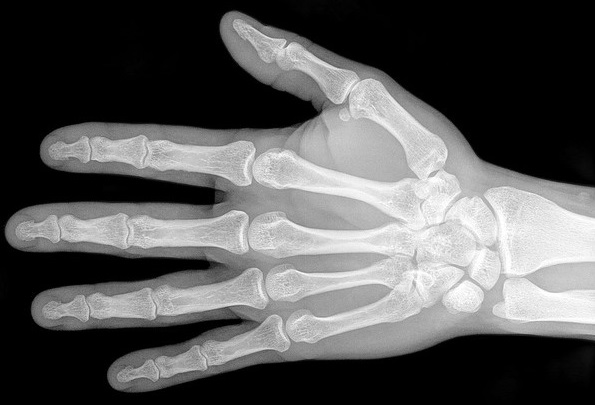
\includegraphics[width=\linewidth]{img/xrayhand.jpg}
  \caption{X-ray image of a human hand. In this negative image, bones are
  lighter because fewer X-rays managed to get through them.}
  \label{fig:xrayhand}
\end{center}
\end{figure}

\subsection{History}
Radiography - and indeed many other imaging modalities - build on the work of
Wilhelm Konrad R\"ontgen, a German physicist who produced and detected X-rays
for the first time on 8 November 1895. These X-rays (X for unknown) had the
remarkable property of being attenuated at different rates when passing through
various materials. For example, bone strongly attenuates the X-rays while soft
tissue does much less so. R\"ontgen also discovered that the radiation can be
captured on a photographic plate, just like regular light. He presented his
findings in his paper ``On a new kind or rays'' \cite{rontgen}. This discovery
earned him the Nobel Prize in Physics in 1901.

Only two weeks after his discovery he produced the first X-ray photo of his
wife's hand, after which she reportedly exclaimed: ``I have seen my death!''.
Just a couple of months later, X-rays were already being used in a clinical
setting on patients.

\subsection{Technical background}
To better understand the internal workings of imaging devices, we present a
simplified mathematical and physical background based on the book of prof.
Suetens\cite{suetens}. X-rays are simply a form of electromagnetic waves
consisting of photons with a wavelength $\lambda$ on the order of Angstr\o ms
($10^{-10}$m). The corresponding frequency $f$ places these rays firmly in the
ionizing (radioactive) part of the spectrum. The energy of such a wave can be
calculated with the following formula, where $c$ is the speed of light and $h$
is Planck's constant.

\begin{equation}
	E = hf = \frac{hc}{\lambda}.
\end{equation}

X-rays are generated in an X-ray tube, a vacuum tube consisting of a cathode and
an anode Current flowing through the cathode releases electrons,
which are accelerated toward the anode by an applied voltage. Once the electrons
hit the anode, they release part of their energy in the form of X-ray photons.

The attenuation of X-rays through materials can easily be modeled using an
attenuation coefficient $\mu$. The beam intensity when passed through a
homogeneous material of depth $d$ is given by: 

\begin{equation}
	I_{out} = I_{in} e^{-\mu d}.
\end{equation}

To capture X-rays, a detector is needed. Traditionally, a screen-film detector
was used. The familiar photographic film alone is very inefficient
at capturing X-rays: only about 2\% of all photons are absorped. Because X-rays
are radioactive, the applied dose cannot simply be increased to improve the
image quality. Instead, an intensifier screen is used in front of the film. This
screen contains heavy chemical elements, whose electrons are excited by the
incoming photons. When returning to their original state, these electrons emit
more photons that can be captured by the film, raising the absorption efficiency
to about 50\%.

\subsubsection{Digital radiography}
Relatively recently, X-ray systems have moved away from analogue detectors
towards digital ones. Much like digital photographs, digital X-ray scans are far
easier to store, copy, post-process and share. On top of that, they typically
have a much wider exposure range making them more tolerant to over- and
underexposure. These detector systems use storage phosphors to temporarily hold
the absorped radiation instead of immediately releasing it in the form of
photons. This phenomenon is caused by electron traps in the doped material.
Later, this phophor can be read out pixel-wise using an optical detector array
and a laser that gives the eletrons enough energy to escape their trap. The main
obstacle for this paradigm shift was the large pixel size. Pixels of 1 mm make
it much more difficult for a radiologist to analyze the image in its digital
form. Only by the time pixels could be as small as 0.1 mm did the medical world
embrace digital detectors \cite{review}.

Even newer devices use active matrix flat panel detectors. These detectors are
able to produce near real time images where storage phosphors and older
technlogies required minutes or more of processing time. %TODO how?

\subsubsection{A note on digital image quality}
The quality of a digital image can be expressed in three dimensions: resolution,
contrast and noise \cite{suetens}.

Resolution is sometimes simply stated as the pixel density (dots per inch).
However, this only provides an upper bound because in practise neighbouring
pixels can be correlated. For example, due to the imperfect nature of the
recording equipment, a single point can appear as blurred blob on the resulting
image. This blob is called the Point Spread Function (PSF), and is a better
measure for the actual image resolution. If the resolution is isotropic, the
Line Spread Function (LSF) - measured in distinguishable line pairs per mm
(lp/mm) - can also be used. Alternatively, the Optical Transfer Function (OTF,
sometimes also MTF) representing amplitude and phase shifts of a sinusoidal
target can be used. In fact, this OTF is nothing more than the Fourier transform
of the PSF or LSF.

Second, contrast is the intensity difference between neighbouring regions of the
image. More formally, contrast at a given frequency is the amplitude component
of the image at that frequency in the frequency domain (calculated using the
Fourier transform). Contrast is dependent on the whole imaging proces, but also
on the size and shape of the objects in the image.

Third, noise is partly the result of interfering processes. Yet, it is also
inherent to the electromagnetic radiation itself because the waves themselves
are stochastic processes. An important measure is the Signal to Noise Ratio
(SNR) or more appropriately Contrast to Noise Ratio (CNR). Noise can be
estimated by examining the result of an scan with no object present, a so-called
flat-field image. Another measure for the amount of noise is the Wiener
spectrum.

In addition to these three elements, sometimes artefacts appear on scans. The
causes of these artificial image features vary widely depending on the image
modality used and can also be caused by excessive post-processing.

\subsection{Future expectations}
Ever since CT and MRI scanners made their way into hospitals, they have taken
over many of the tasks traditionally reserved for basic radiography. This
declining trend is expected to continue in the foreseeable future.

\section{X-ray computed tomography}
One step up from basic radiography is computed tomography (Greek for ``slice
writing''). The goal here is to create image slices of patients in the
cross-sectional plane rather than the frontal plane. To accomplish this, the X-ray
source-detector pair is rotated around the patient. From this raw data, a
so-called backprojection algorithm can reconstruct the whole cross section
image. A computer is needed to make sense of the output, hence the
\emph{computed} in the name. \autoref{fig:ctscan} shows an example of a chest
CT scan.

\begin{figure}[ht]
\begin{center}
  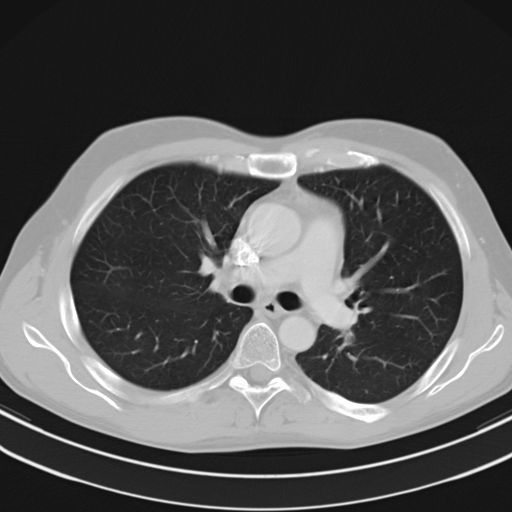
\includegraphics[width=0.4\linewidth]{img/ct-thorax.jpg}
  \caption{Example of a thoracic CT scan. The heart is clearly visible in the
  center. Bones (ribs, sternum, spine) are also easy to spot in the periphery.
  The large black area represents the lungs filled with air.}
  \label{fig:ctscan}
\end{center}
\end{figure}

\subsection{History}
In 1917, Johann Radon - an Austrian mathematician - presented the first
algorithm to reconstruct a function from its projections: the Radon transform
\cite{radon}.

In the 1960's, the South African Allan McLeod Cormack continued working on
the mathematics invented by Radon. A decade later, in 1972, the first
operational CT scanner was designed by Godfrey Hounsfield, an Englishman. They
both received the 1979 Nobel Prize in Physiology and Medicine for their work
related to CT scans.

%helical, 1989
%multislice, 1998

\begin{figure}[ht]
\begin{center}
  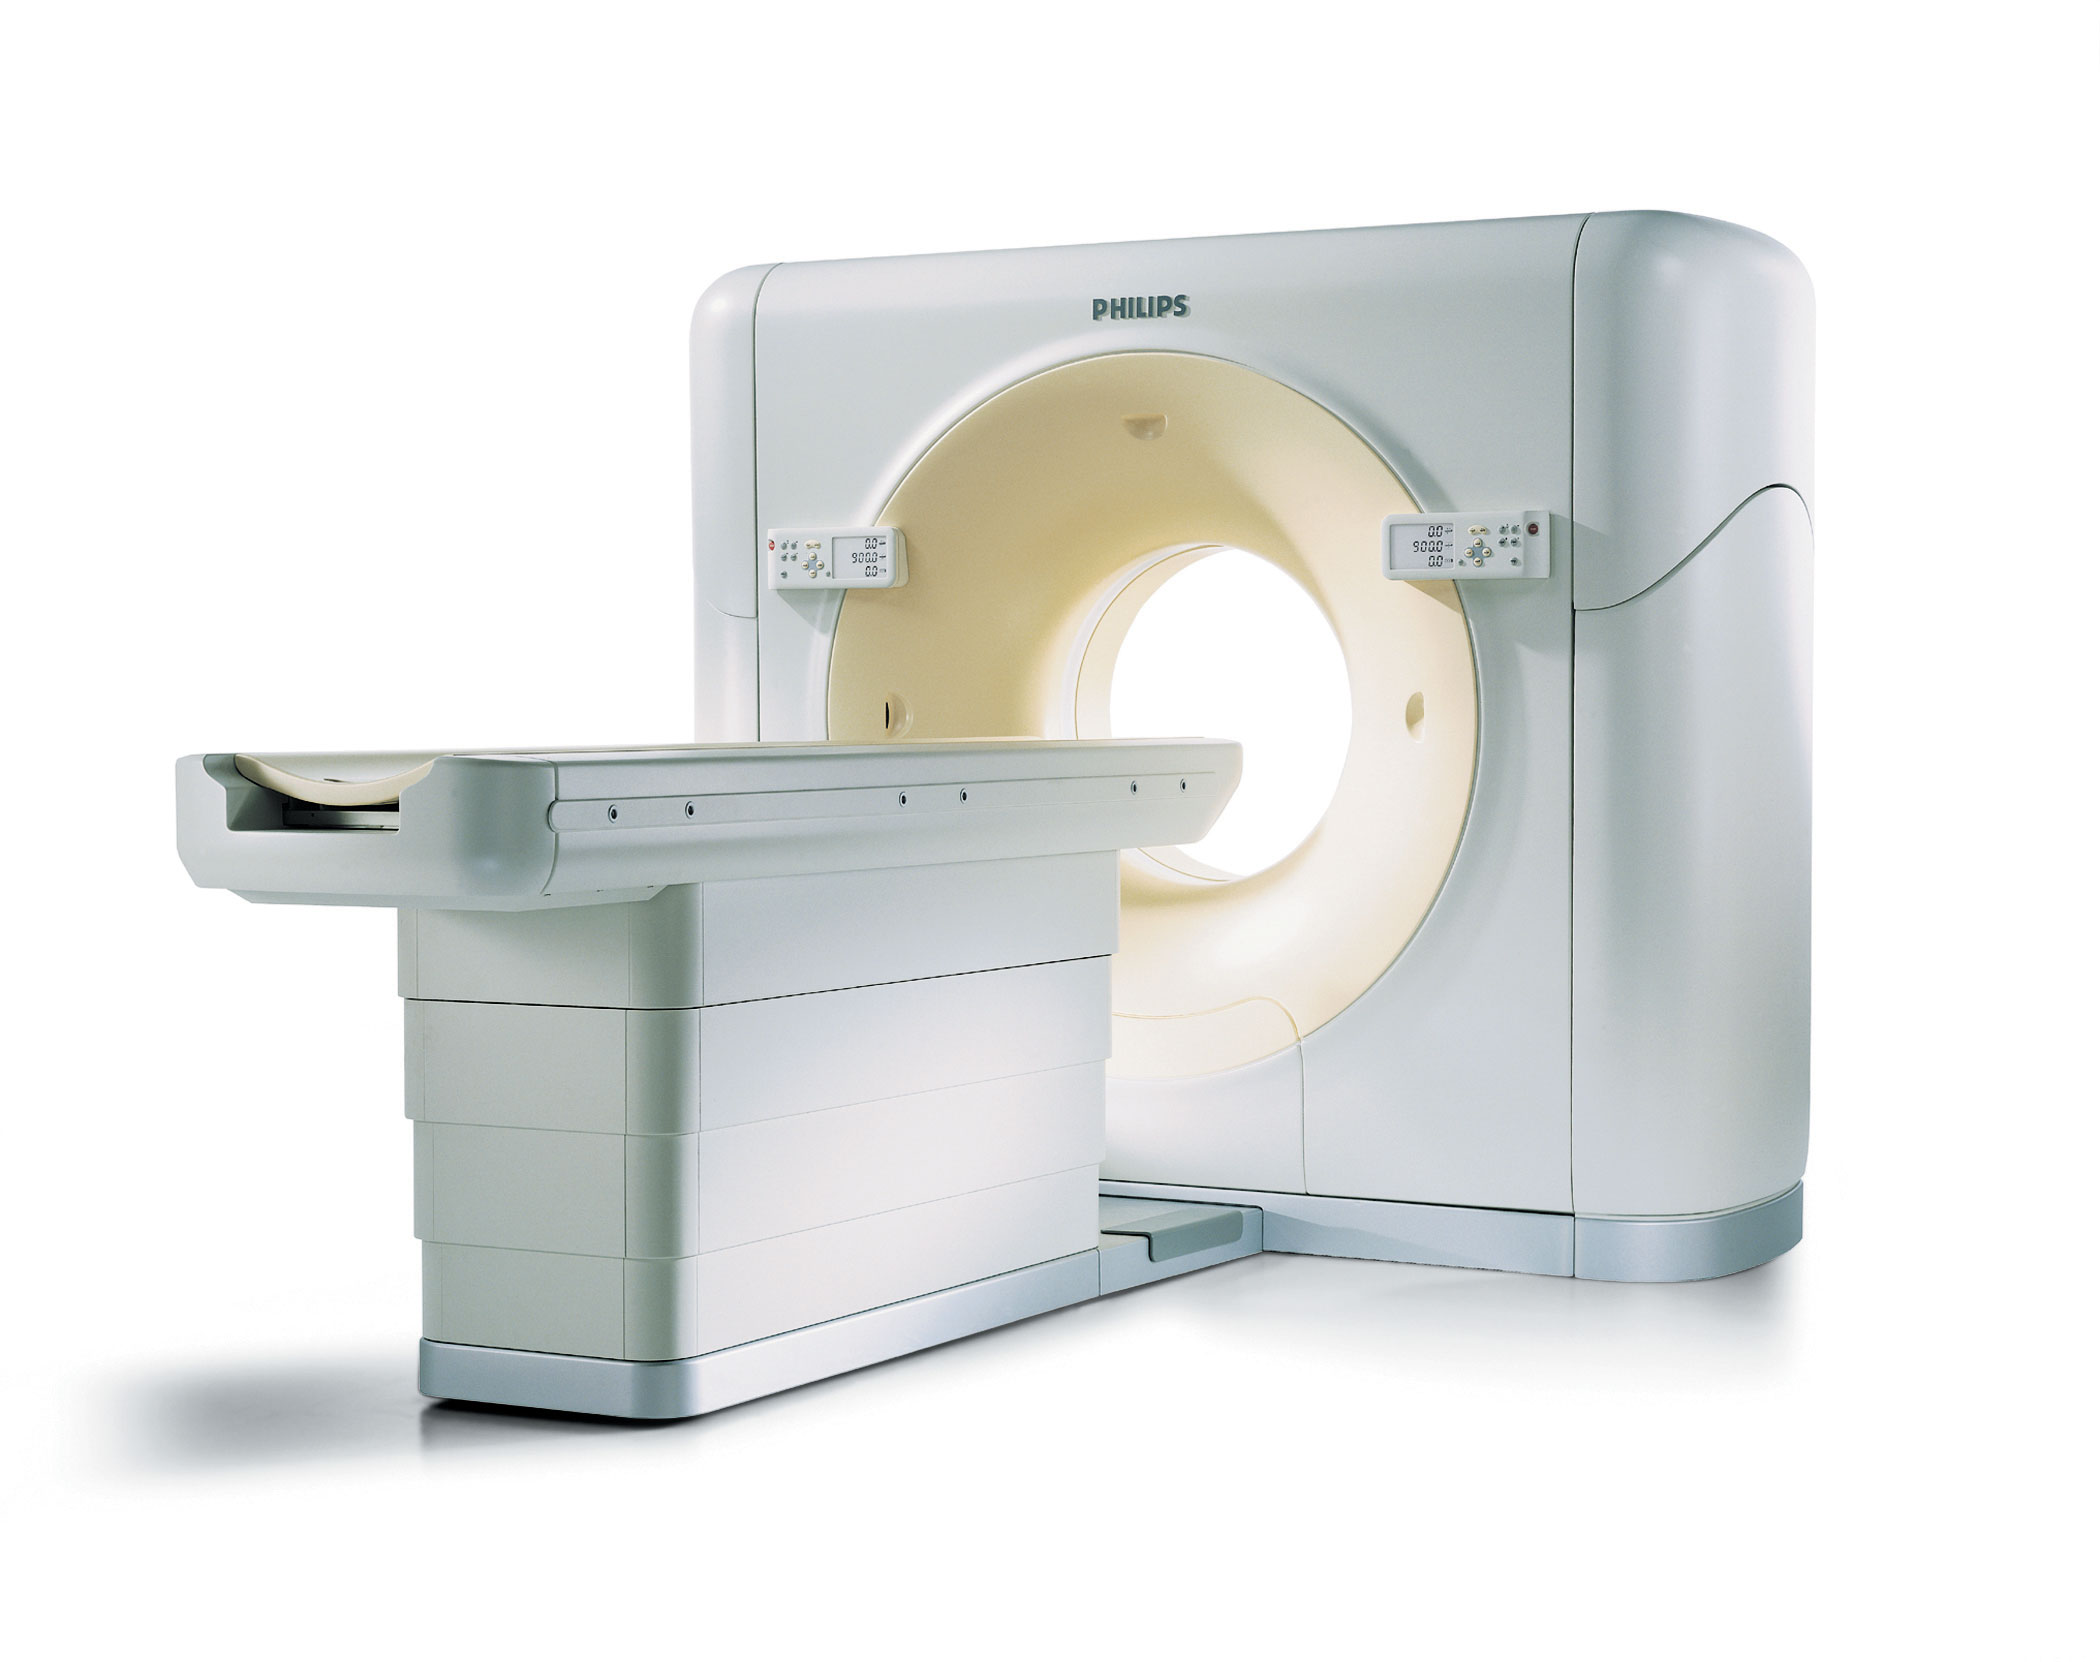
\includegraphics[width=\linewidth]{img/ctscanner.jpg}
  \caption{A CT scanner made by Philips. The patient takes place on the table
  and slowly slides through the toroid wherein the rotating X-ray
  source-detector pair is embedded.}
  \label{fig:ctscanner}
\end{center}
\end{figure}

\subsection{Technical background}

\subsection{Future expectations}

\section{Magnetic resonance imaging}

\subsection{History}

\subsection{Technical background}

\subsection{Future expectations}

\section{Nuclear medicine imaging}

\subsection{History}

\subsection{Technical background}

\subsection{Future expectations}

%ultrasound, img processing, automated diagnosis

%ROC
